\section{Test}
Dies ist ein erster Test.

\subsection{Test 2}
Subsektion, Jockel.

\subsubsection{Dies ist die erste Subsubsection}

Hallo, 1234. Test ÄÖÜ?ßß

ßß ss SS

ß
"s
\section{Zweite Sektion}
Leon stinkt.

\begin{align}
    a^2+b^2                        & =c^2                                               \\
    (a+b)^2                        & =a^2+2ab+b^2                                       \\
    \sum \sum_{n = 1}^{\infty}                                                          \\
    \int_{0}^{2} x^2 \,\mathrm{d}x & = F(x)       & = \frac{x^3}{3} & = F(2) & = 2.6666
\end{align}

Wird hier jetzt auto compiled? Wahrscheinlich nicht. Dies ist ein weiterer Test. Wäre hier nicht Lorem Ipsum besser?

\section{Mathematik}

In dieser Sektion werden Formeln und sonstiges getestet.

\begin{align}
    \label{eq:C}
    x    & =y    & X    & =Y    & a   & =b+c \\
    \label{eq:D}
    x'   & =y'   & X'   & =Y'   & a'  & =b   \\
    \label{eq:F}
    x+x' & =y+y' & X+X' & =Y+Y' & a'b & =c'b
\end{align}

\begin{align}
    x & = y_1-y_2+y_3-y_5+y_8-\dots
      &                             & \text{by~\eqref{eq:C}}                          \\
      & = y'\circ y^*               &                        & \text{by~\eqref{eq:D}} \\
      & = y(0) y'                   &                        & \text {by Axiom 1.}
\end{align}

\begin{equation}
    E = mc^2
\end{equation}

\begin{multline}
    \framebox[.65\columnwidth]{A}\\
    \framebox[.5\columnwidth]{B}\\
    \shoveright{\framebox[.55\columnwidth]{C}}\\
    \framebox[.65\columnwidth]{D}
\end{multline}

\section{Grafiken}

\begin{figure}[h]
    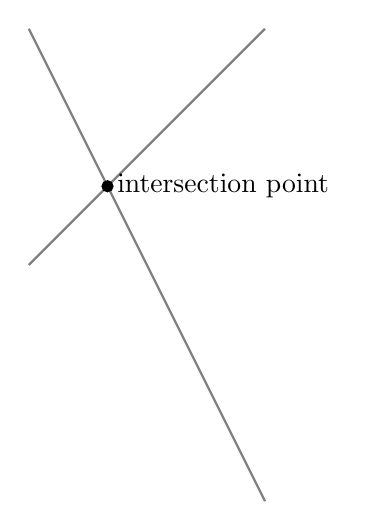
\begin{tikzpicture}
        \draw[gray, thick] (-1, 2) -- (2, -4);
        \draw[gray, thick] (-1, -1) -- (2, 2);
        \filldraw[black] (0,0) circle (2pt) node[anchor=west]{intersection point};
    \end{tikzpicture}
\end{figure}

\begin{figure}[h]
    \begin{tikzpicture}
        \draw (-2,0) -- (2,0);
        \filldraw[gray] (0,0) circle (2pt);
        \draw (-2,-2) .. controls (0,0) .. (2,-2);
        \draw (-2,2) .. controls (-1,0) and (1,0) ..(2,2);
    \end{tikzpicture}
\end{figure}

% \begin{figure}[h]
%     \begin{tikzpicture}
%         \filldraw[color=red!60, fill=red!5, very thick](-1,0) circle (1.5);
%         \fill[blue!50] (2.5,0) ellipse (1.5 and 0.5);
%         \draw[ultra thick, ->] (6.5,0) arc (0:220:1);
%     \end{tikzpicture}
% \end{figure}

% \begin{figure}[h]
%     \begin{tikzpicture}[scale=0.9]
%         \draw[ultra thick]
%         (0,1.5) -- (0,2.5) -- (5,2.5) -- (5,1.5) node[below]{Empfänger};
%         \draw[ultra thick]
%         (0,1) -- (0,0) -- (5,0) -- (5,1);
%         \draw
%         (0,1.5) node[below]{Sender};
%         \path[thick, ->]
%         (1,0) edge (1,2.5);
%         \draw (1,1.25) node[right]{5V};
%     \end{tikzpicture}        
% \end{figure}

Dies ist ein weiterer Test.

Und hier noch mehr Text (oder Tests).

\newpage